\documentclass[border=7pt]{standalone}
\usepackage{fontspec,unicode-math}
\setmainfont{Noto Serif}
\setmathfont{STIXTwoMath-Regular.otf}
\usepackage{tikz}
\usetikzlibrary{arrows.meta,calc,patterns,decorations.markings,decorations.pathmorphing,decorations.pathreplacing}
\tikzset{lev/.style={line width=1.1pt,line cap=butt},
 fine/.style={line width=.52pt},light/.style={line width=.35pt},
 curve/.style={line width=1.15pt,line cap=round,line join=round},
 ax/.style={line width=.57pt,-{Latex[length=2mm,width=1.15mm]}},
 ray/.style={line width=.58pt,-{Latex[length=1.9mm,width=1mm]},shorten >=1.2pt,shorten <=1.2pt},
 dim/.style={line width=.50pt,{Latex[length=1.65mm,width=.85mm]}-{Latex[length=1.65mm,width=.85mm]}},
 flow/.style={line width=.65pt,postaction={decorate},decoration={markings,mark=at position .6 with {\arrow{Latex[length=1.8mm,width=.95mm]}}}},
 lab/.style={font=\fontsize{12}{14.4}\selectfont,inner sep=1.5pt},
 small/.style={font=\fontsize{10.5}{12.5}\selectfont,inner sep=1.2pt},
 panel/.style={font=\fontsize{12}{14.4}\selectfont\itshape,inner sep=1.5pt}}
\pagestyle{empty}
\begin{document}
% CP15: two source-traced molecular potential terms. Not fitted ab initio energies.
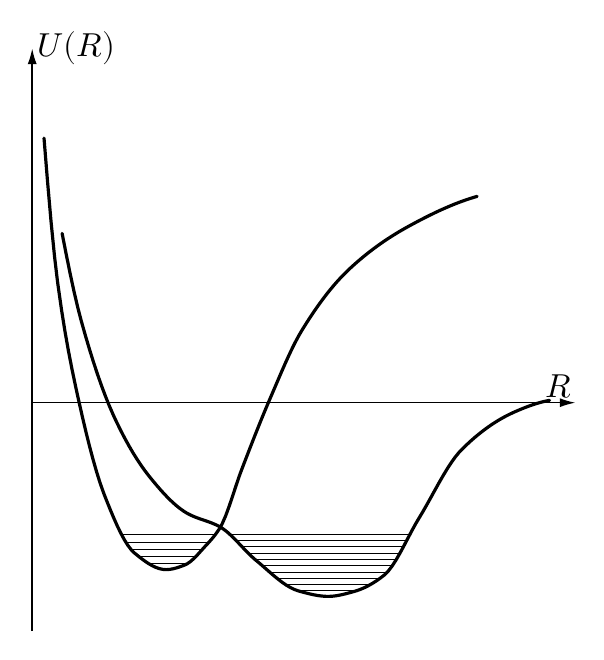
\begin{tikzpicture}[x=1cm,y=1cm,line join=round]
\draw[ax] (0,-2.90)--(0,4.50) node[lab,right] {$U(R)$};
\draw[ax] (0,0)--(6.90,0) node[lab,above left] {$R$};
\draw[light] (1.47294,-2.04000)--(1.97863,-2.04000);
\draw[light] (1.34906,-1.95000)--(2.08187,-1.95000);
\draw[light] (1.25108,-1.86000)--(2.16363,-1.86000);
\draw[light] (1.18789,-1.77000)--(2.24639,-1.77000);
\draw[light] (1.13711,-1.68000)--(2.32253,-1.68000);
\draw[light] (3.38000,-2.39000)--(4.11370,-2.39000);
\draw[light] (3.21642,-2.31000)--(4.29449,-2.31000);
\draw[light] (3.10873,-2.23000)--(4.41785,-2.23000);
\draw[light] (3.01407,-2.15000)--(4.51190,-2.15000);
\draw[light] (2.92261,-2.07000)--(4.57412,-2.07000);
\draw[light] (2.82799,-1.99000)--(4.62511,-1.99000);
\draw[light] (2.74248,-1.91000)--(4.67097,-1.91000);
\draw[light] (2.66557,-1.83000)--(4.71420,-1.83000);
\draw[light] (2.58966,-1.75000)--(4.75622,-1.75000);
\draw[light] (2.50817,-1.67000)--(4.79812,-1.67000);
% CP15 visually traced author curve A; source: F19_4.jpg
\draw[curve] plot coordinates {(0.15000,3.36000) (0.19435,2.81332) (0.23871,2.30731) (0.28306,1.86152) (0.32000,1.55000) (0.32742,1.49427) (0.37177,1.18323) (0.41613,0.90571) (0.46048,0.65593) (0.50484,0.42787) (0.54919,0.21574) (0.57000,0.12000) (0.59355,0.01352) (0.63790,-0.18184) (0.68226,-0.36929) (0.72661,-0.54736) (0.77097,-0.71472) (0.81532,-0.86991) (0.85968,-1.01159) (0.90403,-1.13830) (0.92000,-1.18000) (0.94839,-1.25181) (0.99274,-1.36164) (1.03710,-1.46711) (1.08145,-1.56649) (1.12581,-1.65810) (1.17016,-1.74022) (1.21452,-1.81116) (1.25887,-1.86919) (1.30000,-1.91000) (1.30323,-1.91267) (1.34758,-1.94881) (1.39194,-1.98337) (1.43629,-2.01561) (1.48065,-2.04483) (1.52500,-2.07027) (1.56935,-2.09124) (1.61371,-2.10700) (1.65806,-2.11682) (1.70000,-2.12000) (1.70242,-2.11999) (1.74677,-2.11692) (1.79113,-2.10900) (1.83548,-2.09723) (1.87984,-2.08261) (1.92419,-2.06613) (1.94000,-2.06000) (1.96855,-2.04612) (2.01290,-2.01505) (2.05726,-1.97500) (2.10161,-1.92894) (2.14597,-1.87977) (2.19032,-1.83049) (2.20000,-1.82000) (2.23468,-1.78274) (2.27903,-1.73336) (2.32339,-1.67888) (2.36774,-1.61589) (2.39000,-1.58000) (2.41210,-1.53903) (2.45645,-1.43752) (2.50081,-1.31688) (2.54516,-1.18522) (2.58952,-1.05050) (2.63387,-0.92082) (2.66000,-0.85000) (2.67823,-0.80258) (2.72258,-0.68750) (2.76694,-0.57309) (2.81129,-0.45973) (2.85565,-0.34770) (2.90000,-0.23739) (2.94435,-0.12910) (2.98871,-0.02314) (3.02000,0.05000) (3.03306,0.08030) (3.07742,0.18395) (3.12177,0.28784) (3.16613,0.39092) (3.21048,0.49203) (3.25484,0.59012) (3.29919,0.68404) (3.34355,0.77272) (3.38790,0.85503) (3.42000,0.91000) (3.43226,0.93011) (3.47661,1.00146) (3.52097,1.07061) (3.56532,1.13750) (3.60968,1.20215) (3.65403,1.26451) (3.69839,1.32460) (3.74274,1.38236) (3.78710,1.43780) (3.83145,1.49089) (3.87581,1.54163) (3.92016,1.58997) (3.96452,1.63593) (4.00887,1.67946) (4.02000,1.69000) (4.05323,1.72087) (4.09758,1.76094) (4.14194,1.79975) (4.18629,1.83732) (4.23065,1.87371) (4.27500,1.90892) (4.31935,1.94302) (4.36371,1.97605) (4.40806,2.00802) (4.45242,2.03899) (4.49677,2.06898) (4.54113,2.09804) (4.58548,2.12619) (4.62984,2.15349) (4.67419,2.17996) (4.71855,2.20565) (4.76290,2.23058) (4.78000,2.24000) (4.80726,2.25487) (4.85161,2.27880) (4.89597,2.30238) (4.94032,2.32556) (4.98468,2.34833) (5.02903,2.37065) (5.07339,2.39250) (5.11774,2.41384) (5.16210,2.43465) (5.20645,2.45489) (5.25081,2.47455) (5.29516,2.49358) (5.33952,2.51197) (5.38387,2.52967) (5.42823,2.54667) (5.47258,2.56292) (5.51694,2.57842) (5.56129,2.59311) (5.60565,2.60698) (5.65000,2.62000)};
% CP15 visually traced author curve B; source: F19_4.jpg
\draw[curve] plot coordinates {(0.38000,2.15000) (0.42992,1.89459) (0.47984,1.64894) (0.52976,1.41755) (0.57968,1.20493) (0.62000,1.05000) (0.62960,1.01526) (0.67952,0.83934) (0.72944,0.67154) (0.77935,0.51208) (0.82927,0.36108) (0.87919,0.21876) (0.92911,0.08530) (0.97903,-0.03910) (1.02895,-0.15426) (1.05000,-0.20000) (1.07887,-0.26071) (1.12879,-0.36158) (1.17871,-0.45728) (1.22863,-0.54785) (1.27855,-0.63335) (1.32847,-0.71379) (1.37839,-0.78923) (1.42831,-0.85971) (1.47823,-0.92526) (1.49000,-0.94000) (1.52815,-0.98691) (1.57806,-1.04674) (1.62798,-1.10443) (1.67790,-1.15950) (1.72782,-1.21151) (1.77774,-1.26000) (1.82766,-1.30453) (1.87758,-1.34464) (1.92750,-1.37989) (1.96000,-1.40000) (1.97742,-1.40982) (2.02734,-1.43466) (2.07726,-1.45561) (2.12718,-1.47398) (2.17710,-1.49107) (2.22702,-1.50817) (2.27694,-1.52659) (2.32685,-1.54762) (2.37677,-1.57257) (2.39000,-1.58000) (2.42669,-1.60351) (2.47661,-1.64223) (2.52653,-1.68712) (2.57645,-1.73643) (2.62637,-1.78842) (2.67629,-1.84135) (2.72621,-1.89348) (2.77613,-1.94306) (2.82605,-1.98835) (2.84000,-2.00000) (2.87597,-2.02994) (2.92589,-2.07285) (2.97581,-2.11654) (3.02573,-2.16013) (3.07565,-2.20273) (3.12556,-2.24347) (3.17548,-2.28148) (3.22540,-2.31588) (3.27532,-2.34578) (3.32524,-2.37031) (3.37516,-2.38859) (3.38000,-2.39000) (3.42508,-2.40266) (3.47500,-2.41610) (3.52492,-2.42852) (3.57484,-2.43946) (3.62476,-2.44851) (3.67468,-2.45521) (3.72460,-2.45914) (3.76000,-2.46000) (3.77452,-2.45981) (3.82444,-2.45652) (3.87435,-2.44968) (3.92427,-2.44004) (3.97419,-2.42832) (4.02411,-2.41528) (4.07403,-2.40164) (4.08000,-2.40000) (4.12395,-2.38665) (4.17387,-2.36830) (4.22379,-2.34657) (4.27371,-2.32145) (4.32363,-2.29296) (4.37355,-2.26110) (4.42347,-2.22587) (4.47000,-2.19000) (4.47339,-2.18724) (4.52331,-2.13704) (4.57323,-2.07130) (4.62315,-1.99326) (4.67306,-1.90622) (4.72298,-1.81340) (4.77290,-1.71808) (4.82282,-1.62352) (4.87274,-1.53300) (4.91000,-1.47000) (4.92266,-1.44927) (4.97258,-1.36466) (5.02250,-1.27660) (5.07242,-1.18661) (5.12234,-1.09621) (5.17226,-1.00691) (5.22218,-0.92022) (5.27210,-0.83768) (5.32202,-0.76078) (5.37194,-0.69105) (5.42185,-0.63002) (5.45000,-0.60000) (5.47177,-0.57832) (5.52169,-0.53024) (5.57161,-0.48440) (5.62153,-0.44076) (5.67145,-0.39931) (5.72137,-0.36001) (5.77129,-0.32283) (5.82121,-0.28775) (5.87113,-0.25474) (5.92105,-0.22376) (5.97097,-0.19480) (6.02089,-0.16781) (6.07081,-0.14278) (6.12000,-0.12000) (6.12073,-0.11968) (6.17065,-0.09791) (6.22056,-0.07706) (6.27048,-0.05728) (6.32040,-0.03874) (6.37032,-0.02158) (6.42024,-0.00597) (6.47016,0.00794) (6.52008,0.01998) (6.57000,0.03000)};
\end{tikzpicture}
\end{document}
